\documentclass[11pt,a4paper]{report}
\usepackage[textwidth=37em,vmargin=30mm]{geometry}
\usepackage{calc,xunicode,amsmath,amssymb,paralist,enumitem,tabu,booktabs,datetime2,xeCJK,xeCJKfntef,listings}
\usepackage{tocloft,fancyhdr,tcolorbox,xcolor,graphicx,eso-pic,xltxtra,xelatexemoji}

\newcommand{\envyear}[0]{2025}
\newcommand{\envdatestr}[0]{2025-06-20}
\newcommand{\envfinaldir}[0]{webdb/2025/20250620/final}

\usepackage[hidelinks]{hyperref}
\hypersetup{
    colorlinks=false,
    pdfpagemode=FullScreen,
    pdftitle={Web Digest - \envdatestr}
}

\setlength{\cftbeforechapskip}{10pt}
\renewcommand{\cftchapfont}{\rmfamily\bfseries\large\raggedright}
\setlength{\cftbeforesecskip}{2pt}
\renewcommand{\cftsecfont}{\sffamily\small\raggedright}

\setdefaultleftmargin{2em}{2em}{1em}{1em}{1em}{1em}

\usepackage{xeCJK,xeCJKfntef}
\xeCJKsetup{PunctStyle=plain,RubberPunctSkip=false,CJKglue=\strut\hskip 0pt plus 0.1em minus 0.05em,CJKecglue=\strut\hskip 0.22em plus 0.2em}
\XeTeXlinebreaklocale "zh"
\XeTeXlinebreakskip = 0pt


\setmainfont{Brygada 1918}
\setromanfont{Brygada 1918}
\setsansfont{IBM Plex Sans}
\setmonofont{JetBrains Mono NL}
\setCJKmainfont{Noto Serif CJK SC}
\setCJKromanfont{Noto Serif CJK SC}
\setCJKsansfont{Noto Sans CJK SC}
\setCJKmonofont{Noto Sans CJK SC}

\setlength{\parindent}{0pt}
\setlength{\parskip}{8pt}
\linespread{1.15}

\lstset{
	basicstyle=\ttfamily\footnotesize,
	numbersep=5pt,
	backgroundcolor=\color{black!5},
	showspaces=false,
	showstringspaces=false,
	showtabs=false,
	tabsize=2,
	captionpos=b,
	breaklines=true,
	breakatwhitespace=true,
	breakautoindent=true,
	linewidth=\textwidth
}






\newcommand{\coverpic}[2]{
    % argv: itemurl, authorname
    Cover photo by #2~~(\href{#1}{#1})
}
\newcommand{\makeheader}[0]{
    \begin{titlepage}
        % \newgeometry{hmargin=15mm,tmargin=21mm,bmargin=12mm}
        \begin{center}
            
            \rmfamily\scshape
            \fontspec{BaskervilleF}
            \fontspec{Old Standard}
            \fontsize{59pt}{70pt}\selectfont
            WEB\hfill DIGEST
            
            \vfill
            % \vskip 30pt
            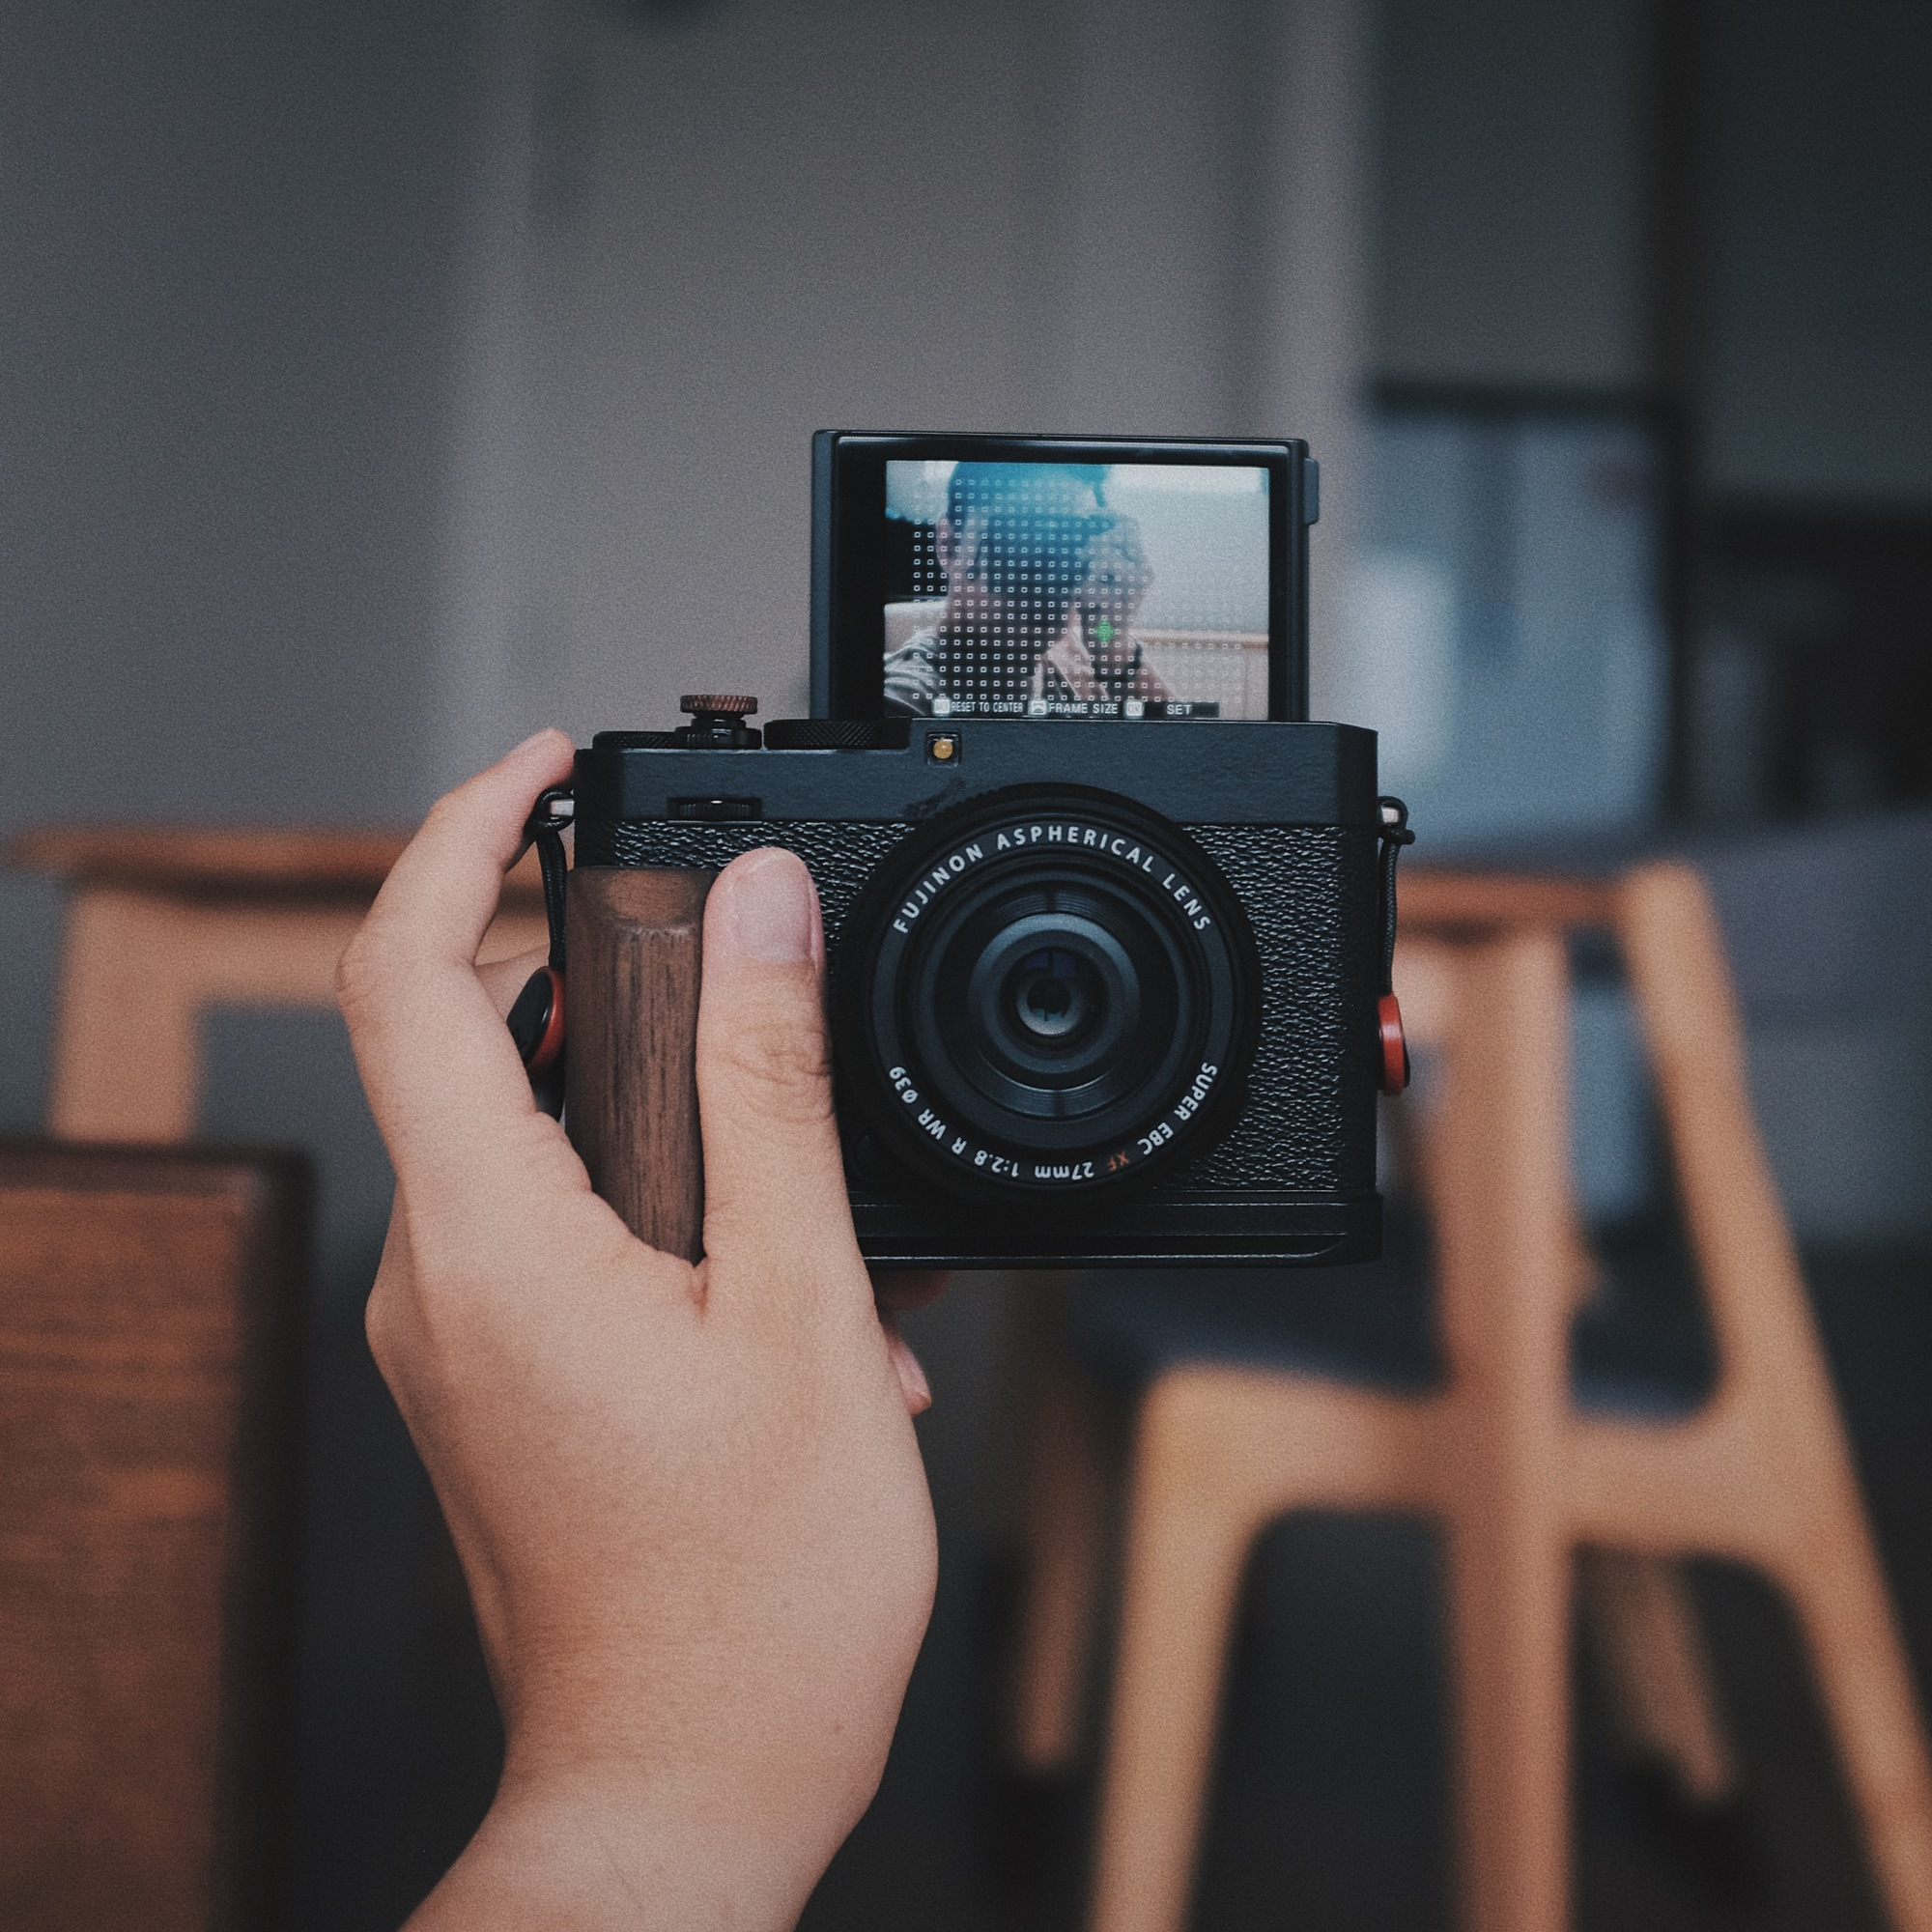
\includegraphics[width=\linewidth]{\envfinaldir/coverpic-prod.jpg}\par
            % \vskip 30pt
            \vfill

            \normalsize\rmfamily\scshape
            \copyright{} The Web Digest Project \hfill\large \envdatestr
        \end{center}
    \end{titlepage}
    % \restoregeometry
}
\newcommand{\simplehref}[1]{%
    \textcolor{blue!80!green}{\href{#1}{#1}}%
}
\renewcommand{\contentsname}{\center\Huge\sffamily\bfseries Contents\par\vskip 20pt}
\newcounter{ipartcounter}
\setcounter{ipartcounter}{0}
\newcommand{\ipart}[1]{
    % \vskip 20pt
    \clearpage
    \stepcounter{ipartcounter}
    \phantomsection
    \addcontentsline{toc}{chapter}{#1}
    % \begin{center}
    %     \Huge
    %     \sffamily\bfseries
    %     #1
    % \end{center}
    % \vskip 20pt plus 7pt
}
\newcounter{ichaptercounter}
\setcounter{ichaptercounter}{0}
\newcommand{\ichapter}[1]{
    % \vskip 20pt
    \clearpage
    \stepcounter{ichaptercounter}
    \phantomsection
    \addcontentsline{toc}{section}{\numberline{\arabic{ichaptercounter}}#1}
    \begin{center}
        \Huge
        \sffamily\bfseries
        #1
    \end{center}
    \vskip 20pt plus 7pt
}
\newcommand{\entrytitlefont}[1]{\subsection*{\raggedright\Large\sffamily\bfseries#1}}
\newcommand{\entryitemGeneric}[2]{
    % argv: title, url
    \parbox{\linewidth}{
        \entrytitlefont{#1}\par\vskip 5pt
        \footnotesize\ttfamily\mdseries
        \simplehref{#2}
    }\vskip 11pt plus 11pt minus 1pt
}
\newcommand{\entryitemGithub}[3]{
    % argv: title, url, desc
    \parbox{\linewidth}{
        \entrytitlefont{#1}\par\vskip 5pt
        \footnotesize\ttfamily\mdseries
        \simplehref{#2}\par\vskip 5pt
        \small\rmfamily\mdseries#3
    }\vskip 11pt plus 11pt minus 1pt
}
\newcommand{\entryitemAp}[3]{
    % argv: title, url, desc
    \parbox{\linewidth}{
        \entrytitlefont{#1}\par\vskip 5pt
        \footnotesize\ttfamily\mdseries
        \simplehref{#2}\par\vskip 5pt
        \small\rmfamily\mdseries#3
    }\vskip 11pt plus 11pt minus 1pt
}
\newcommand{\entryitemHackernews}[3]{
    % argv: title, hnurl, rawurl
    % \parbox{\linewidth}{
    %     \entrytitlefont{#1}\par\vskip 5pt
    %     \footnotesize\ttfamily\mdseries
    %     \simplehref{#3}\par
    %     \textcolor{black!50}{\href{#2}{#2}}
    % }\vskip 11pt plus 11pt minus 1pt
    \begin{minipage}{\linewidth}
            \entrytitlefont{#1}\par\vskip 5pt
            \footnotesize\ttfamily\mdseries
            \simplehref{#3}\par
            \textcolor{black!50}{\href{#2}{#2}}
    \end{minipage}\par\vskip 11pt plus 11pt minus 1pt
}







\begin{document}

\makeheader

\tableofcontents\clearpage




\ipart{Developers}
\ichapter{Hacker News}
\entryitemTwoLinks{Estrogen: A Trip Report}{https://news.ycombinator.com/item?id=44322153}{https://smoothbrains.net/posts/2025-06-15-estrogen.html}

\entryitemTwoLinks{Compiling LLMs into a MegaKernel: A path to low-latency inference}{https://news.ycombinator.com/item?id=44321672}{https://zhihaojia.medium.com/compiling-llms-into-a-megakernel-a-path-to-low-latency-inference-cf7840913c17}

\entryitemTwoLinks{Juneteenth in Photos}{https://news.ycombinator.com/item?id=44320851}{https://texashighways.com/travel-news/the-history-of-juneteenth-in-photos/}

\entryitemTwoLinks{In praise of ``normal'' engineers}{https://news.ycombinator.com/item?id=44320806}{https://charity.wtf/2025/06/19/in-praise-of-normal-engineers/}

\entryitemTwoLinks{Curved-Crease Sculpture}{https://news.ycombinator.com/item?id=44318874}{https://erikdemaine.org/curved/}

\entryitemTwoLinks{Show HN: A DOS-like hobby OS written in Rust and x86 assembly}{https://news.ycombinator.com/item?id=44318588}{https://github.com/krustowski/rou2exOS}

\entryitemTwoLinks{End of 10: Upgrade your old Windows 10 computer to Linux}{https://news.ycombinator.com/item?id=44318420}{https://endof10.org/}

\entryitemTwoLinks{What would a Kubernetes 2.0 look like}{https://news.ycombinator.com/item?id=44317825}{https://matduggan.com/what-would-a-kubernetes-2-0-look-like/}

\entryitemTwoLinks{Guess I'm a Rationalist Now}{https://news.ycombinator.com/item?id=44317180}{https://scottaaronson.blog/?p=8908}

\entryitemTwoLinks{Show HN: Claude Code Usage Monitor – real-time tracker to dodge usage cut-offs}{https://news.ycombinator.com/item?id=44317012}{https://github.com/Maciek-roboblog/Claude-Code-Usage-Monitor}

\entryitemTwoLinks{Base44 sells to Wix for \$80M cash}{https://news.ycombinator.com/item?id=44316920}{https://techcrunch.com/2025/06/18/6-month-old-solo-owned-vibe-coder-base44-sells-to-wix-for-80m-cash/}

\entryitemTwoLinks{From LLM to AI Agent: What's the Real Journey Behind AI System Development?}{https://news.ycombinator.com/item?id=44316909}{https://www.codelink.io/blog/post/ai-system-development-llm-rag-ai-workflow-agent}

\entryitemTwoLinks{SpaceX Starship 36 Anomaly}{https://news.ycombinator.com/item?id=44315529}{https://twitter.com/NASASpaceflight/status/1935548909805601020}

\entryitemTwoLinks{Elliptic Curves as Art}{https://news.ycombinator.com/item?id=44315321}{https://elliptic-curves.art/}

\entryitemTwoLinks{Dr. Demento Announces Retirement After 55-Year Radio Career}{https://news.ycombinator.com/item?id=44315185}{https://sopghreporter.com/2025/06/01/dr-demento-announces-retirement/}

\entryitemTwoLinks{I feel open source has turned into two worlds}{https://news.ycombinator.com/item?id=44315179}{https://utcc.utoronto.ca/~cks/space/blog/tech/OpenSourceTwoWorlds}

\entryitemTwoLinks{The Zed Debugger Is Here}{https://news.ycombinator.com/item?id=44314977}{https://zed.dev/blog/debugger}

\entryitemTwoLinks{TI to invest \$60B to manufacture foundational semiconductors in the U.S.}{https://news.ycombinator.com/item?id=44314759}{https://www.ti.com/about-ti/newsroom/news-releases/2025/texas-instruments-plans-to-invest-more-than--60-billion-to-manufacture-billions-of-foundational-semiconductors-in-the-us.html}

\entryitemTwoLinks{Andrej Karpathy: Software in the era of AI [video]}{https://news.ycombinator.com/item?id=44314423}{https://www.youtube.com/watch?v=LCEmiRjPEtQ}

\entryitemTwoLinks{MCP Specification – version 2025-06-18 changes}{https://news.ycombinator.com/item?id=44314289}{https://modelcontextprotocol.io/specification/2025-06-18/changelog}


\ipart{Developers~~~~(zh-Hans)}
\ichapter{Solidot}
\entryitemGeneric{\hskip 0pt{}城市人造光源的规模有多大}{https://www.solidot.org/story?sid=81600}

\entryitemGeneric{\hskip 0pt{}SpaceX 的 Starship 36 在静态点火测试中爆炸}{https://www.solidot.org/story?sid=81599}

\entryitemGeneric{\hskip 0pt{}石油巨头面临首宗气候死亡诉讼}{https://www.solidot.org/story?sid=81598}

\entryitemGeneric{\hskip 0pt{}秸秆覆盖大幅增加竹林土壤碳排放}{https://www.solidot.org/story?sid=81597}

\entryitemGeneric{\hskip 0pt{}媒体竞争如何驱动虚假信息传播}{https://www.solidot.org/story?sid=81596}

\entryitemGeneric{\hskip 0pt{}美国新签证规定要求留学生将社媒账号设为公开}{https://www.solidot.org/story?sid=81595}

\entryitemGeneric{\hskip 0pt{} AI教父辛顿最新访谈:在个性化算法时代,人类的共同体验消失了,数字智能必然超越生物智能,但20\%的灭绝概率正被忽视}{https://www.solidot.org/story?sid=81594}

\entryitemGeneric{\hskip 0pt{}微生物被发现有类似病毒的特征}{https://www.solidot.org/story?sid=81593}

\entryitemGeneric{\hskip 0pt{}微软报告晚上八点后开会的次数在增加}{https://www.solidot.org/story?sid=81592}

\entryitemGeneric{\hskip 0pt{}Netflix 纪录片揭露 OceanGate 泰坦号潜艇事故的更多细节}{https://www.solidot.org/story?sid=81591}

\entryitemGeneric{\hskip 0pt{}伊朗禁止官员使用联网设备}{https://www.solidot.org/story?sid=81590}

\entryitemGeneric{\hskip 0pt{}生活在受微塑料污染的海边可能增加心血管代谢疾病风险 }{https://www.solidot.org/story?sid=81589}

\entryitemGeneric{\hskip 0pt{}使用大模型如何影响你的大脑}{https://www.solidot.org/story?sid=81588}

\entryitemGeneric{\hskip 0pt{}AMD 宣布 CDNA 4 架构}{https://www.solidot.org/story?sid=81587}

\entryitemGeneric{\hskip 0pt{}本田成功测试可重复使用火箭}{https://www.solidot.org/story?sid=81586}

\entryitemGeneric{\hskip 0pt{}为什么中国拥抱开源?}{https://www.solidot.org/story?sid=81585}

\entryitemGeneric{\hskip 0pt{}特朗普第三次给予 TikTok 90 天宽限期}{https://www.solidot.org/story?sid=81584}

\entryitemGeneric{\hskip 0pt{}伊朗计划全面断网}{https://www.solidot.org/story?sid=81583}

\entryitemGeneric{\hskip 0pt{}科学家创造出一种致命真菌去对抗蚊子}{https://www.solidot.org/story?sid=81582}

\entryitemGeneric{\hskip 0pt{}研究人员创造出第一种完全可验证的真随机数生成器}{https://www.solidot.org/story?sid=81581}\ichapter{V2EX}
\entryitemGeneric{\hskip 0pt{}[程序员] 斐讯 N1 如何走局域网内 windows 上的代理软件代理流量?}{https://www.v2ex.com/t/1139799}

\entryitemGeneric{\hskip 0pt{}[OpenAI] Thiings}{https://www.v2ex.com/t/1139797}

\entryitemGeneric{\hskip 0pt{}[Telegram] Telegram 创始人 Pavel Durov 最近接受的一次采访:我不喝茶和咖啡,也不吃糖}{https://www.v2ex.com/t/1139796}

\entryitemGeneric{\hskip 0pt{}[Cursor] 寄了寄了, Cursor Pro 完全没法用高级模型了,这咋整啊。。。}{https://www.v2ex.com/t/1139795}

\entryitemGeneric{\hskip 0pt{}[分享创造] Proxifier v4.14 汉化分享,给你更顺畅的中文体验 🍃}{https://www.v2ex.com/t/1139792}

\entryitemGeneric{\hskip 0pt{}[云计算] 腾讯云 EdgeOne 推出 ``全球首个支持中国访问的免费 CDN''}{https://www.v2ex.com/t/1139791}

\entryitemGeneric{\hskip 0pt{}[程序员] 在搞一个站点翻译,将 wxt 文档翻译成中文}{https://www.v2ex.com/t/1139789}

\entryitemGeneric{\hskip 0pt{}[V2EX 站点状态] 20250619 - 10 分钟左右的停服维护}{https://www.v2ex.com/t/1139788}

\entryitemGeneric{\hskip 0pt{}[iPhone] 真的假的:外版 iPhone 能自动把 LiveCommunicationKit 转换成 CallKit,锁屏时直接相当于接电话,只是仍然不会留存通话记录}{https://www.v2ex.com/t/1139787}

\entryitemGeneric{\hskip 0pt{}[程序员] 独立开发者\&创业者的大家是怎么找到交流圈子的}{https://www.v2ex.com/t/1139786}

\entryitemGeneric{\hskip 0pt{}[Windows] wslg 尝试安装桌面后非常卡顿}{https://www.v2ex.com/t/1139784}

\entryitemGeneric{\hskip 0pt{}[问与答] 短信服务}{https://www.v2ex.com/t/1139783}

\entryitemGeneric{\hskip 0pt{}[分享发现] 2025-06 B 站的视频大部分都只有 30hz 了}{https://www.v2ex.com/t/1139782}

\entryitemGeneric{\hskip 0pt{}[怀旧游戏] xemu 项目进展神速}{https://www.v2ex.com/t/1139781}

\entryitemGeneric{\hskip 0pt{}[酷工作] [伦敦 AI 初创企业] 高级 AI 工程师( Python )}{https://www.v2ex.com/t/1139780}

\entryitemGeneric{\hskip 0pt{}[问与答] 尼康 Z30 有办法将相机内存卡中的照片自动增量同步到 NAS 中吗?}{https://www.v2ex.com/t/1139779}

\entryitemGeneric{\hskip 0pt{}[职场话题] 想问个问题,关于工作的}{https://www.v2ex.com/t/1139778}

\entryitemGeneric{\hskip 0pt{}[Apple] 求救: RealVNC Viewer 远程 MAC 的时候挺卡的,局域网,还有那个鼠标轮动距离特别小}{https://www.v2ex.com/t/1139777}

\entryitemGeneric{\hskip 0pt{}[程序员] 国内哪个产商的 ddos 价格划算一些}{https://www.v2ex.com/t/1139776}

\entryitemGeneric{\hskip 0pt{}[Apple] 你以为的 esim 普及能够带来新的体验!}{https://www.v2ex.com/t/1139775}

\entryitemGeneric{\hskip 0pt{}[硬件] 有没有和戴尔 KB216 键盘一样手感,但是 是 87 键的薄膜键盘?}{https://www.v2ex.com/t/1139774}

\entryitemGeneric{\hskip 0pt{}[宽带症候群] 上海联通有因为用 ddns 被封宽带的吗?}{https://www.v2ex.com/t/1139773}

\entryitemGeneric{\hskip 0pt{}[Web3] 现在还适合 web 3.0 么}{https://www.v2ex.com/t/1139772}

\entryitemGeneric{\hskip 0pt{}[宽带症候群] 上海电信精品网刚才突然断线后只能拨到 218.80 段的 IP}{https://www.v2ex.com/t/1139770}

\entryitemGeneric{\hskip 0pt{}[macOS] mac 电脑有没有可以运行 flash 游戏的浏览器}{https://www.v2ex.com/t/1139769}

\entryitemGeneric{\hskip 0pt{}[钓鱼] 玩路亚之后,鱼没上两条,装备买了一堆,纯经验分享一波}{https://www.v2ex.com/t/1139767}

\entryitemGeneric{\hskip 0pt{}[生活] 记一次以失败而告终的小区(集体)维权经历}{https://www.v2ex.com/t/1139766}

\entryitemGeneric{\hskip 0pt{}[奇思妙想] 劳动者的企业制度革命-基于区块链的动态股权合作社制度设计}{https://www.v2ex.com/t/1139765}

\entryitemGeneric{\hskip 0pt{}[旅行] 都在计划暑假旅游了,我也跟一个,打算带对象广州出发,走广西-云南-广州环线}{https://www.v2ex.com/t/1139764}

\entryitemGeneric{\hskip 0pt{}[Windows] 重装系统无限蓝屏}{https://www.v2ex.com/t/1139762}

\entryitemGeneric{\hskip 0pt{}[程序员] 开源 | Feishu MCP Server:让 AI 工具 (Cursor/ChatWise/Windsurf......) 真正「无感」接入飞书文档}{https://www.v2ex.com/t/1139761}

\entryitemGeneric{\hskip 0pt{}[分享发现] 大上 paperlike13kf 录制了几秒的视频效果。}{https://www.v2ex.com/t/1139759}

\entryitemGeneric{\hskip 0pt{}[Electron] mac 程序签名公证问题}{https://www.v2ex.com/t/1139757}

\entryitemGeneric{\hskip 0pt{}[投资] 分享一个最近的稳健机会}{https://www.v2ex.com/t/1139756}

\entryitemGeneric{\hskip 0pt{}[新手求助] 不懂就问这是什么神秘代码}{https://www.v2ex.com/t/1139755}

\entryitemGeneric{\hskip 0pt{}[程序员] 如果产品 PRD 是 prompt, LLM 输出技术方案, Figma MCP+Cursor 编写代码, browner-user agent 功能测试}{https://www.v2ex.com/t/1139753}

\entryitemGeneric{\hskip 0pt{}[推广] 有没有需要开源项目广告位的}{https://www.v2ex.com/t/1139752}

\entryitemGeneric{\hskip 0pt{}[远程工作] 招聘<远程>前端}{https://www.v2ex.com/t/1139751}

\entryitemGeneric{\hskip 0pt{}[酷工作] [杭州] 支付宝招前端}{https://www.v2ex.com/t/1139750}

\entryitemGeneric{\hskip 0pt{}[汽车] 老哥们,车顶架有木有推荐的哈}{https://www.v2ex.com/t/1139747}

\entryitemGeneric{\hskip 0pt{}[Apple] 5202 年了,还有人用 airdrop 安装 IPA 么?}{https://www.v2ex.com/t/1139746}

\entryitemGeneric{\hskip 0pt{}[分享创造] 裸眼 3D 文字海报生成器}{https://www.v2ex.com/t/1139744}

\entryitemGeneric{\hskip 0pt{}[问与答] 请问下用国内的服务器搭建 NTP 服务器,违法吗?会被 ban 吗?}{https://www.v2ex.com/t/1139743}

\entryitemGeneric{\hskip 0pt{}[程序员] 专为 Claude Code 设计的基于 YAML 的 Playwright UI 自动化测试}{https://www.v2ex.com/t/1139741}

\entryitemGeneric{\hskip 0pt{}[职场话题] 刚入职场,经常压力自己,怎么解?}{https://www.v2ex.com/t/1139740}

\entryitemGeneric{\hskip 0pt{}[职场话题] 诚恳找数据分析实习}{https://www.v2ex.com/t/1139739}

\entryitemGeneric{\hskip 0pt{}[求职] [济南]找工作,十四年一线技术老鸟}{https://www.v2ex.com/t/1139738}

\entryitemGeneric{\hskip 0pt{}[西安] 帮忙给下西安游的建议}{https://www.v2ex.com/t/1139737}

\entryitemGeneric{\hskip 0pt{}[程序员] 发现 Python debug 有个问题}{https://www.v2ex.com/t/1139734}

\entryitemGeneric{\hskip 0pt{}[程序员] oschina 已经沦为 广告社区,付费推广社区,自吹自擂社区,是否有同类替代网站推荐?}{https://www.v2ex.com/t/1139730}


\ipart{Generic News}







\clearpage
\leavevmode\vfill
\footnotesize

Copyright \copyright{} 2023-2025 Neruthes and other contributors.

This document is published with CC BY-NC-ND 4.0 license.

The entries listed in this newsletter may be copyrighted by their respective creators.

This newsletter is generated by the Web Digest project.

The newsletters are also delivered via Telegram channel \CJKunderline{\href{https://t.me/webdigestchannel}{https://t.me/webdigestchannel}}.\\
RSS feed is available at \CJKunderline{\href{https://webdigest.pages.dev/rss.xml}{https://webdigest.pages.dev/rss.xml}}.

This newsletter is available in PDF at
\CJKunderline{\href{https://webdigest.pages.dev/}{https://webdigest.pages.dev/}}.

The source code being used to generate this newsletter is available at\\
\CJKunderline{\href{https://github.com/neruthes/webdigest}{https://github.com/neruthes/webdigest}}.

This newsletter is also available in
\CJKunderline{\href{http://webdigest.pages.dev/readhtml/\envyear/WebDigest-20250620.html}{HTML}} and
\CJKunderline{\href{https://github.com/neruthes/webdigest/blob/master/markdown/\envyear/WebDigest-20250620.md}{Markdown}}.


\coverpic{https://unsplash.com/photos/a-light-filled-cafe-interior-with-plants-vygFIMTe5l4}{rawkkim}


\end{document}
